
\documentclass[ms.tex]{subfiles}
\begin{document}

\section{Application to Observations}
\label{sec:h3}

% fig 5
\begin{figure*}
\centering
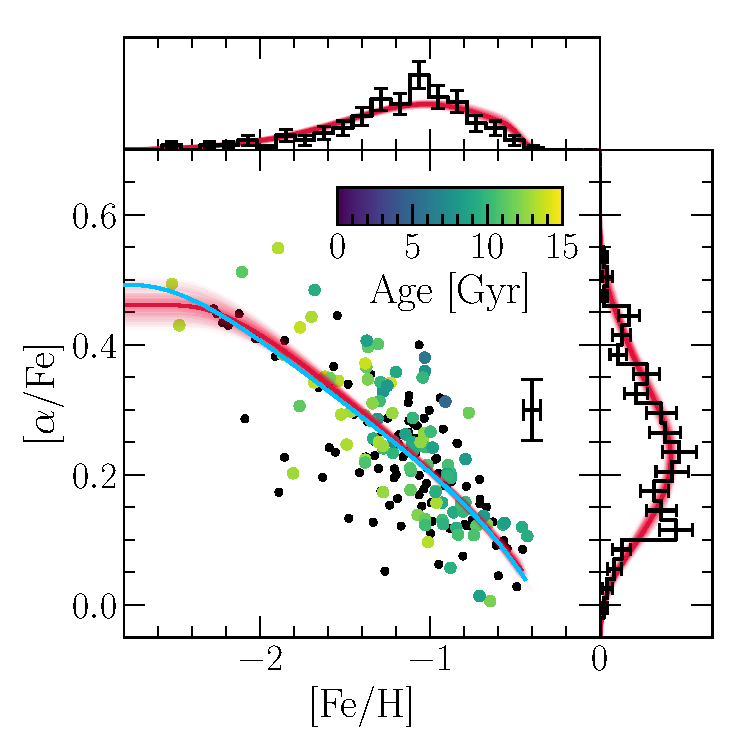
\includegraphics[scale = 0.65]{gsefit_afe_feh.pdf}
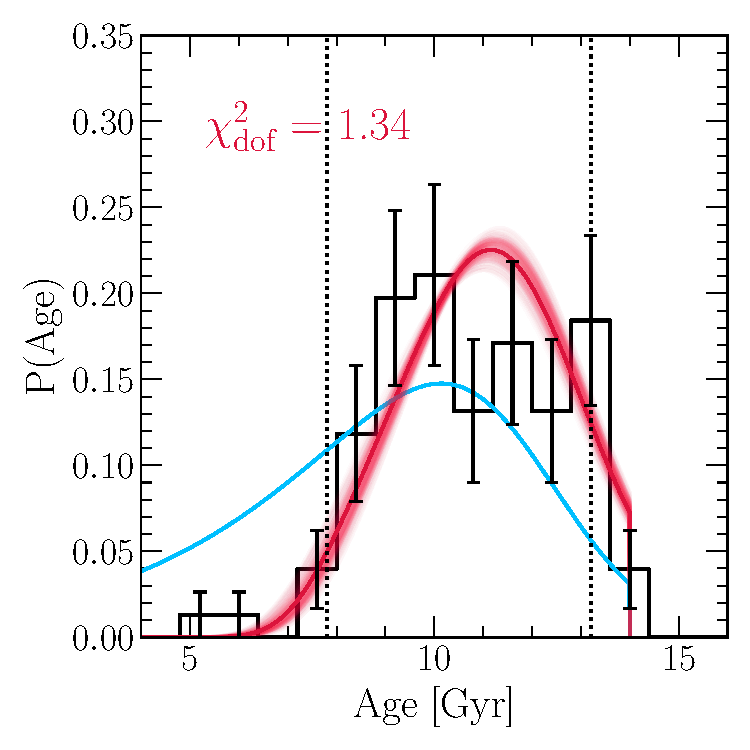
\includegraphics[scale = 0.54]{gsefit_agedist.pdf}
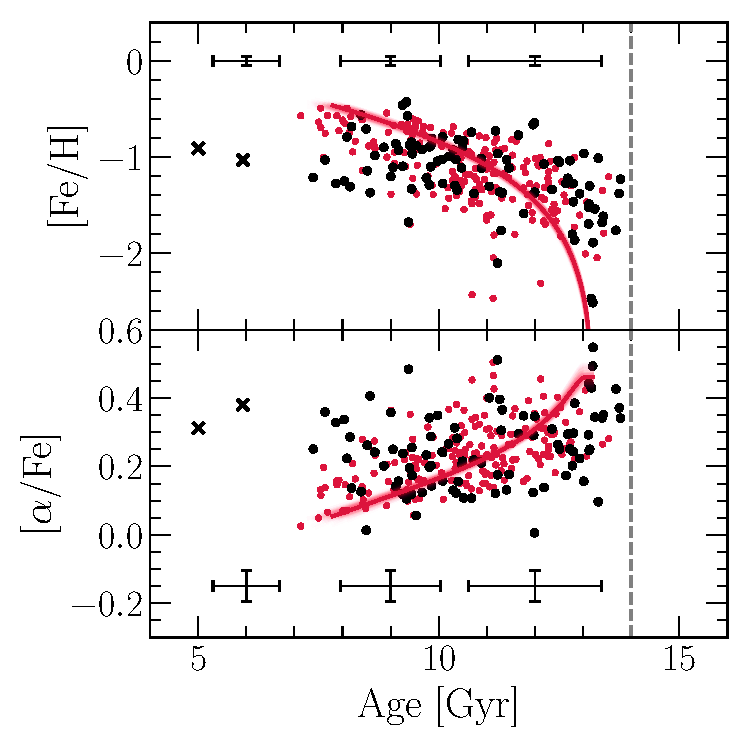
\includegraphics[scale = 0.53]{gsefit_amr.pdf}
\caption{
Our GSE sample.
Red lines in all panels denote the best-fit one-zone model, while the
blue lines in the left and middle panels denote the best-fit model when the
age measurements are excluded from the fit.
Distributions in~\feh,~\afe~and age are convolved with the median uncertainty
of the sample (see discussion in~\S~\ref{sec:h3:gse}).
We additionally subsample 200 sets of parameter choices from our Markov chain
and plot their predictions as highly transparent lines to offer a sense of the
fit uncertainty.
\textbf{Left}: The~\afe-\feh~plane and the associated marginalized
distributions.
Stars are colour-coded according to their ages where available and are
otherwise plotted in black.
The median~\feh~and~\afe~uncertainty in the sample is shown by the error bar
to the right of the data.
Error bars indicate a~$\sqrt{N}$ uncertainty associated with random
sampling both here and in the middle panel.
\textbf{Middle}: The age distribution measured for our GSE sample (black,
binned).
\textbf{Right}: The age-\feh~(top) and age-\afe~(bottom) relations for our
sample (black) and our best-fit chemical evolution model (red).
The median~\feh,~\afe~and age uncertainties are shown by the error bars at the
top and bottom of each panel.
We plot the two stars that we exclude from our fit as black X's (likely
blue stragglers; see discussion in~\S~\ref{sec:h3:gse}).
Red points denote a mock sample drawn from our best-fit model with~$N = 95$
stars (the same size as the stars with ages in our GSE sample) and perturbed by
the median age uncertainty of the sample.
}
\label{fig:gse}
\end{figure*}

% fig 6
\begin{figure*}
\centering
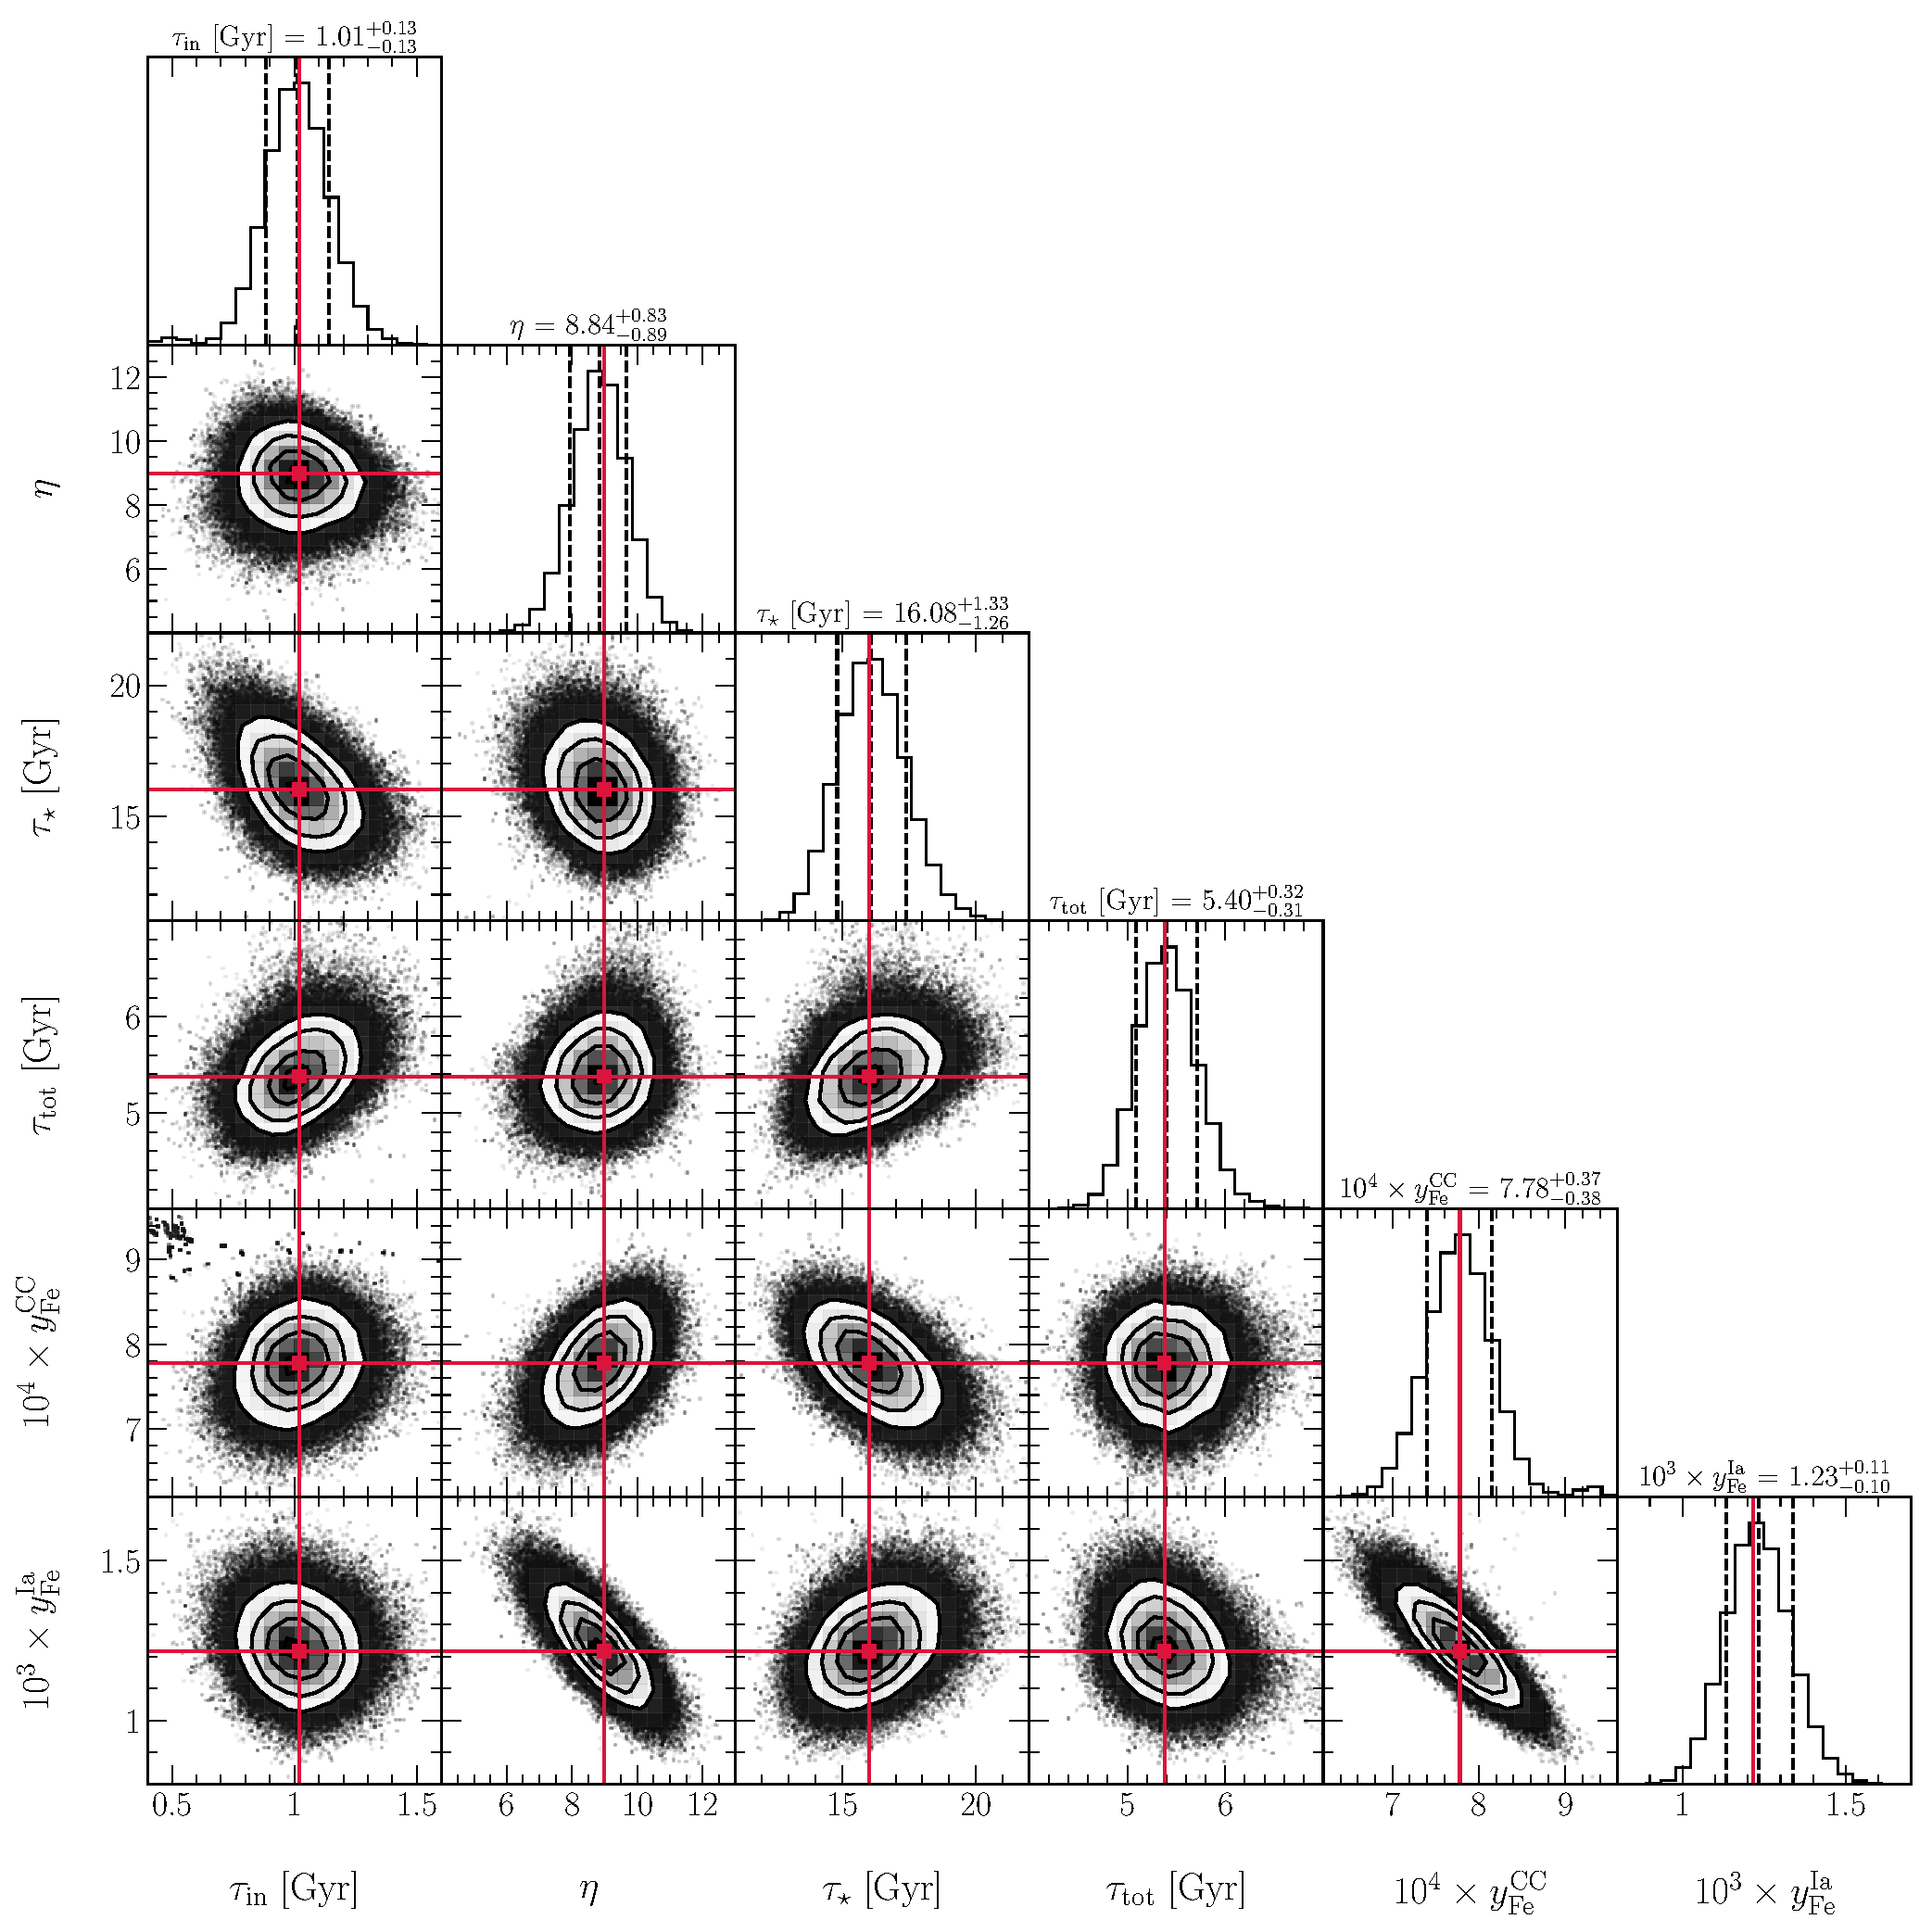
\includegraphics[scale = 0.5]{gsechem_512k.pdf}
\caption{
The ``corner-plot'' showing the results of our fitting method applied to GSE
stars observed by the H3 survey.
Panels below the diagonal show 2-dimensional cross-sections of the likelihood
function while panels along the diagonal show the marginalized distributions
along with the best-fit values and confidence intervals.
Red ``cross-hairs'' mark the element of the Markov chain with the maximum
statistical likelihood.
}
\label{fig:gse_corner}
\end{figure*}

We now apply our likelihood function (equation~\ref{eq:likelihood}) to two
dwarf satellite remnants observed in the Milky Way halo.
The first is a relatively well-studied system: GSE~\citep{Belokurov2018,
Helmi2018}, believed to be responsible for a major merger event early in the
Milky Way's history~\citep{Chaplin2020} which contributed~$10^9 - 10^{10}~\msun$
of total stellar mass to the Galaxy~\citep{Deason2019, Fattahi2019,
Mackereth2019, Vincenzo2019}, including eight globular clusters in the stellar
halo~\citep{Myeong2018}.
The second is a less well-studied system: the Wukong stream, a prograde
structure chemically distinct from the GSE which sits between it and the
Helmi stream~\citep{Helmi1999} in energy-angular momentum space
\citep{Naidu2020, Naidu2022}.
We make use of data from the H3 survey (see discussion
in~\S~\ref{sec:h3:survey} below) and discuss our GCE model fits to GSE and
Wukong in~\S\S~\ref{sec:h3:gse} and~\ref{sec:h3:wukong} below.

\subsection{The H3 Survey}
\label{sec:h3:survey}

The H3 survey~\citep{Conroy2019} is collecting medium-resolution spectra
of~$\sim$300,000 stars in high-latitude fields ($\left|b\right| > 20^\circ$).
Spectra are collected from the Hectochelle instrument on the MMT
\citep{Szentgyorgyi2011} which delivers~$R \approx$~32,000 spectra over the
wavelength range of~$5150 - 5300$~\AA.
Spectral lines in this wavelength range are dominated by iron-peak elements,
but it does safely include the FeI/MgI blended line at 5167~\AA~as well as
the strong MgI lines at 5173 and 5184~\AA~(see Fig. 6 of~\citealt{Conroy2019}).
Throughout this section, the alpha element abundances we refer to are therefore
Mg abundances specifically, whereas in previous sections an alpha element
refers to any species where the only statistically significant enrichment
source is a metallicity-dependent yield from massive stars.
\par
The survey selection function is deliberately simple: the primary sample
consists of stars with~$r$ band magnitudes of~$15 < r < 18$ and Gaia
\citet{Gaia2016} parallaxes~$<$ 0.3 mas (this threshold has evolved over the
course of the survey as the Gaia astrometry has become more precise).
Stellar parameters are estimated by the~\textsc{MINESweeper} program
\citep{Cargile2020}, which fits grids of isochrones, synthetic spectra and
photometry to the Hectochelle spectrum and broadband photometry from Gaia,
Pan-STARRS~\citep{Chambers2016}, SDSS~\citep{York2000}, 2MASS
\citep{Skrutskie2006} and WISE~\citep{Wright2010} with the Gaia parallax
used as a prior.
The fitted parameters include radial velocity, spectrophotometric distance,
reddening,~\feh,~\afe~and age.
The default analysis includes a complicated prior on age and distance
(see~\citealt{Cargile2020} for details).
We have also re-fit high signal-to-noise data with a flat age prior for cases
where ages play an important role.
In this paper we use the catalog which uses this flat age prior.


\subsection{Gaia-Sausage Enceladus}
\label{sec:h3:gse}

\subfile{results.tablebody.tex}

Our sample from GSE contains 189 stars, 95 of which have age measurements.
These stars span metallicity of~$\feh \approx -2.5$ to~$-0.4$ and
$\afe \approx 0$ to~$+0.55$.
Abundance uncertainties range from~$\sim$0.02 to~$0.12$ dex in
both~\feh~and~\afe~with median values near~$\sim$0.05.
Of the stars with age measurements, the youngest is~$\sim$5 Gyr old and the
oldest is~$\sim$13.8 Gyr old.
All inferred ages, however, incorporate a prior imposed by~\textsc{MINESweeper}
which requires all values to be below 14 Gyr~\citep{Cargile2020}, preventing
the log-normal nature of age uncertainties from populating the~$\sim14 - 20$
Gyr range.
Every age measurement has a statistical uncertainty
$\sigma_{\log_{10}(\text{age})} \leq 0.05$, corresponding to a measurement
precision of~$\lesssim$12\%.
Due to the difficulty associated with measuring stellar ages both accurately
and precisely~\citep{Soderblom2010, Chaplin2013}, we adopt this value as the
minimum uncertainty to account for any systematic errors that may be present.
This consequently applies to the whole subset of our sample that has age
measurements.
Because H3 selects targets based only on a magnitude range and maximum
parallax, the selection function in chemical space should be nearly uniform
(i.e.~$\script{S}(\script{M}_j | \{\theta\}) \approx 1$ for all points
$\script{M}_j$ along the evolutionary track).
We therefore take the weights appearing in our likelihood function to be
proportional to the SFR alone (see discussion in~\S~\ref{sec:fitting} and
equations~\ref{eq:likelihood} and~\ref{eq:weights}).
\par
The left panel of Fig.~\ref{fig:gse} shows our sample in the~\afe-\feh~plane
along with the associated marginalized distributions.
The mode of the MDF is near~$\feh \approx -1$ and~$\afe \approx + 0.25$ and
the ``knee'' associated with the onset of SN Ia enrichment is apparent near
$\feh \approx -2$, though there are only a few stars in our sample in this
region of chemical space.
Invoking the equilibrium arguments of~\citet{Weinberg2017}, the knee occurring
at low metallicity and an MDF dominated by low metallicity is indicative of
slow star formation (high~$\tau_\star$) and strong outflows (high~$\eta$),
respectively.
This is expected for a dwarf galaxy progenitor where star formation is
typically slow~\citep[e.g.][]{Hudson2015} and the gravitational potential well
is shallow due to low stellar and halo masses.
Furthermore, the alpha-enhanced mode of the MDF is indicative of an SFH which
was truncated early in the GSE's history before SN Ia enrichment could produce
enough Fe to reach solar~\afe.
This is consistent with the age distribution, shown in the middle panel,
which indicates that the GSE is dominated by old stars ($\gtrsim$8 Gyr).
The truncation of the age distribution likely reflects the quenching of star
formation in the GSE progenitor as a consequence of RAM pressure stripping by
the hot halo of the Milky Way after its first infall~$\sim$10 Gyr ago
\citep{Bonaca2020}.
\par
The age-metallicity relation (AMR; both age-\feh~and age-\afe) has a
considerable amount of scatter, in large part because of the considerable age
uncertainties.
We note the presence of two outliers at ages of~$\sim$5 and~$\sim$6 Gyr, marked
by X's in the right panel of Fig.~\ref{fig:gse}.
These stars have abundances typical of the rest of the GSE population but are
anomalously young.
It's likely that these are blue stragglers: stars which are thought to be made
hotter and more luminous by accretion from a binary companion.
As a result, they occupy a region of the CMD which is normally occupied by much
younger, more massive stars, biasing their age measurements to low values
\citep[e.g.][]{Bond1971, Stryker1993}.
We therefore omit these stars from our fit to the GSE, including only those
which are older than~$\sim$7 Gyr.
\par
The steadily sloped decline of~\afe~with increasing~\feh~and the approximately
monotonic nature of the age-\feh~and age-\afe~relations indicate a smooth
SFH.
If the GSE had experienced a burst in star formation at some point in its
history, this would be accompanied by a sudden increase in~\afe~followed by
a decline back toward the pre-burst value due to the temporarily perturbed
ratio of CCSN and SN Ia rates~\citep{Johnson2020}.
We therefore fit the GSE with a smooth evolutionary model, adopting the same
exponential infall history as the input model to our mock samples described
in~\S~\ref{sec:mocks:fiducial}.
\par
Fig.~\ref{fig:gse_corner} shows the likelihood distribution we obtain for GSE
from our fitting method.
We indeed find that the best-fit evolutionary model implies slow star formation
($\tau_\star \approx 16$ Gyr) and strong outflows ($\eta \approx 9$),
qualitatively similar to our mock samples.
Out fit additionally suggests that the Fe yields are
$\yfecc = \scinote{7.78^{+0.37}_{-0.38}}{-4}$ and
$\yfeia = \scinote{1.23^{+0.11}_{-0.10}}{-3}$ on the scale where the alpha
element yield is fixed at~$\yacc = 0.01$.
These Fe yields suggest that massive stars account for
$\yfecc / (\yfecc + \yfeia) \approx $40\% of the Fe in the universe.
This value may however be influenced by the H3 pipeline~\textsc{MINESweeper}
which enforces a prior that~$\afe \leq +0.6$~\citep{Cargile2020} -- if
the~\afe~plateau in nature occurs near this value, this prior could bias
measurements to low~\afe~ratios.
\par
As discussed in~\S~\ref{sec:mocks:recovered} and quantified in
Appendix~\ref{sec:degeneracy}, these yields are subject to the yield-outflow
degeneracy along with~$\eta$ and~$\tau_\star$, and our adopted value
of~\yacc~is intended only to set some overall scale to these values which can
be adjusted as necessary.
Consequently, only relative rather than absolute values carry any meaning.
In the absence of winds (i.e.~$\eta = 0$) but with otherwise the same
evolutionary parameters, the MDF is predicted to have a peak near
$\feh \approx -0.5$ with a tail toward low metallicity and a sharp cutoff at
higher metallicities.
This comparison indicates that star formation in the GSE progenitor was slow
enough that it would have achieved only~$\sim$one-third solar metallicity
within~$\sim$5.4 Gyr of star formation even with the largest sink term in the
enrichment rates removed.
If star formation instead sped up to~$\tau_\star = 1$ Gyr (the expected SFE if
the GSE progenitor were composed entirely of molecular hydrogen while forming
stars at redshifts of~$z \gtrsim 1$;~\citealp{Tacconi2018}), then the
predicted MDF is still peaked near~$\feh \approx -1$ but is more symmetric and
less skewed toward lower~\feh~as in the GSE data (see Fig.~\ref{fig:gse}).
In order to predict an MDF dominated by solar metallicity stars, this model
requires~\textit{both} weaker outflows and more efficient star formation.
\par
The infall timescale~$\tau_\text{in}$ and the total duration of star formation
$\tau_\text{tot}$ are orthogonal to the yield-outflow degeneracy (see
Appendix~\ref{sec:degeneracy}), indicating that both absolute and relative
values carry meaning.
The infall history is sharp ($\tau_\text{in} \approx 1$ Gyr), as expected given
the alpha-enhanced mode of the MDF.
Star formation lasted~$5.40^{+0.32}_{-0.31}$ Gyr after an onset assumed to
occur at a lookback time of 13.2 Gyr based on the predictions of
the~\textsc{UniverseMachine} semi-analytic model of galaxy formation
(\citealp{Behroozi2019}; see discussion in~\S~\ref{sec:mocks:fiducial}).
This corresponds to the GSE's last episode of star formation occurring
$7.80^{+0.31}_{-0.32}$ Gyr ago, consistent with the truncation of the age
distribution around~$\sim$8 Gyr.

% fig 7
\begin{figure}
\centering
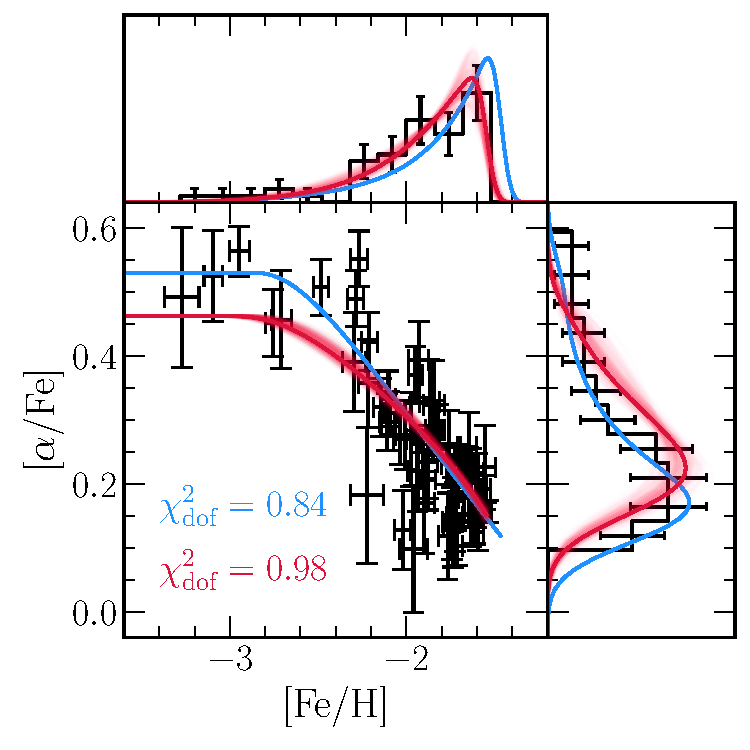
\includegraphics[scale = 0.65]{wukong_bestfit.pdf}
\caption{
Our Wukong sample in the~\afe-\feh~plane and the associated marginalized
distributions.
Error bars in the central denote the measurement uncertainty on individual
stars' abundances, and error bars in the top and right panels indicate the
uncertainty in the abundance distribution assuming~$\sigma = \sqrt{N}$ from
sampling noise.
The red lines denote our best-fit chemical evolution model in red (see
discussion in~\S~\ref{sec:h3:wukong}), with 200 additional sets of parameter
choices subsampled from our Markov chain to give a sense of the fit precision.
The blue lines denote an alternate fit in which we allow the Fe yields to vary
as free parameters.
}
\label{fig:wukong}
\end{figure}

% fig 8
\begin{figure*}
\centering
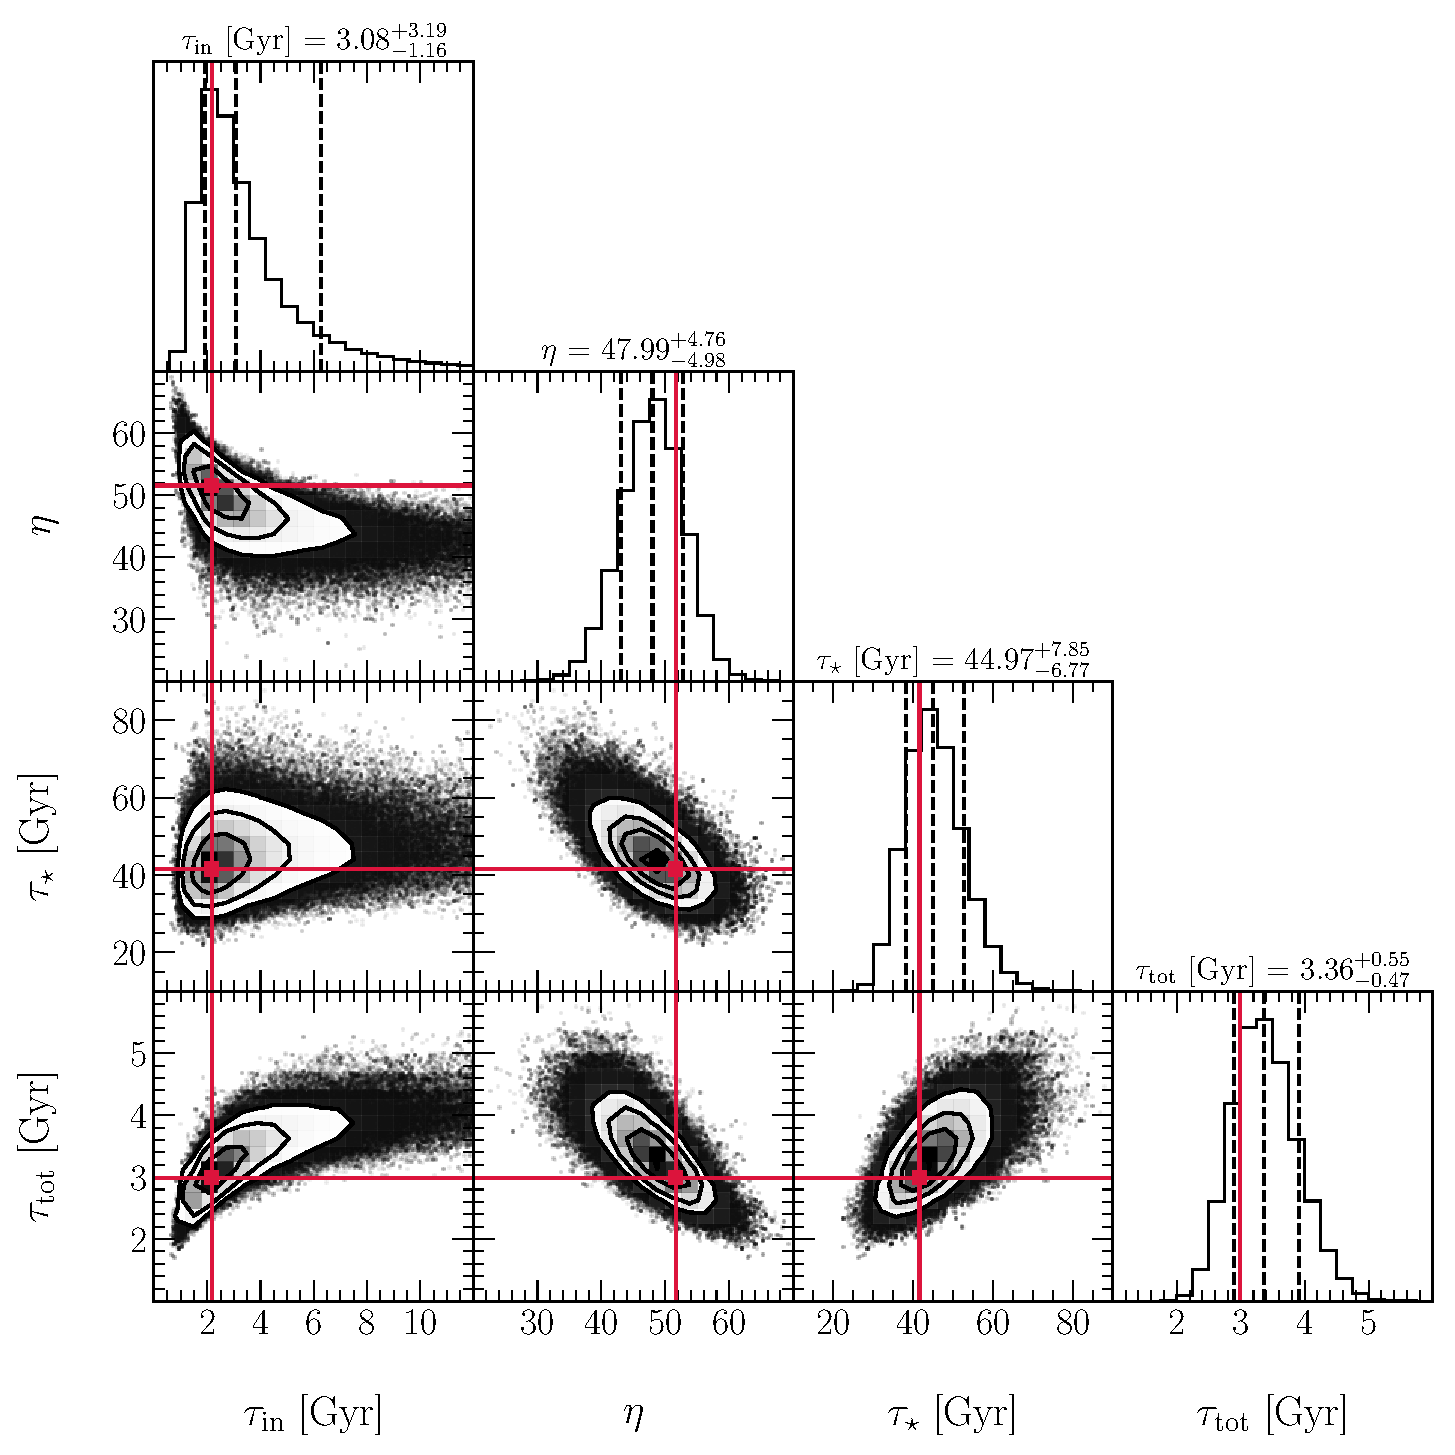
\includegraphics[scale = 0.52]{wukong_512k.pdf}
\caption{
The same as Fig.~\ref{fig:gse_corner} but for our Wukong sample.
In this fit we fix the Fe yields at the values inferred from the GSE sample.
}
\label{fig:wukong_corner}
\end{figure*}

We plot the predictions of our best-fit model over the GSE data in
Fig.~\ref{fig:gse}.
Overall, this model is a reasonable description of the data, but in detail it
predicts a slightly broader~\feh~distribution and a slightly more peaked
age distribution than the data.
We quantify the quality of the fit according to equation
\refp{eq:chisquared_dof}, finding~$\chi_\text{dof}^2 = 1.34$.
As a consequence of the considerable measurement uncertainties in stellar ages,
it might appear at first glance that the model is a poor fit to the
age-\feh~and age-\afe~relations.
To address this, we subsample 95 stars (the same number from our sample that
have age measurements) from our best-fit SFH and perturb their ages and
abundances by the corresponding median uncertainties in the sample and plot the
results in the right panel of Fig.~\ref{fig:gse} for comparison.
The resultant sample occupies a similar region of the age-\feh~and
age-\afe~planes as the data, indicating that the model is indeed a good
description of the GSE.
We do however note an additional~$\sim$6 or 7 potential blue stragglers with
ages of~$\sim8 - 9$ Gyr,~$\feh \approx -1.2$ and~$\afe \approx +0.4$.
These stars are less obviously blue stragglers than the two at ages of 5 or 6
Gyr and would not have stuck out as outliers if we did not have the GCE model
to compare them to.
If we were to remove these stars from our sample, we would expect the quality
of the fit to improve somewhat by lowering the height of the age distribution
at~$\sim8 - 9$ Gyr.
\par
In~\S~\ref{sec:mocks:variations} we found that our model accurately recovered
the known evolutionary timescales of the input model even in the absence of
age information.
However, we fit our mock samples with the exact underlying GCE model and same
numerical code from which they were generated, placing the same systematic
effects in the data as in the model.
In practice, the systematics will generally be different between the two, and
the evolutionary history built into the model is not necessarily a perfect
description of the galaxy.
To demonstrate this, we conduct an additional fit to our GSE sample leaving
out the age measurements.
The SN yields and mass-loading factor inferred in this case are consistent
with our original fit, but in comparison it significantly overestimates the
infall timescale ($\tau_\text{in} = 2.18^{+0.43}_{-0.56}$ Gyr), the SFE
timescale ($\tau_\star = 26.60^{+4.83}_{-6.11}$ Gyr) and the duration of star
formation ($\tau_\text{tot} = 10.73^{+1.76}_{-2.69}$ Gyr).
We show the evolutionary track in chemical space and age distribution predicted
by this model in Fig.~\ref{fig:gse}.
Without any age information, our method achieves an accurate description of the
abundance distributions, but the age distribution is significantly more
extended than the data.
Although our results presented in~\S~\ref{sec:mocks:variations} suggest that it
is theoretically possible to infer GCE model parameters from detailed
abundances without any age information, this comparison suggests that those
measurements are much more important in practice for pinning down evolutionary
timescales.
While the most powerful way to provide this information for the likelihood
function is with individual age measurements, in principle it can also be
achieved with, e.g., constructing a prior based on a CMD-derived SFH as in
\citet{Dolphin2002} and~\citet{Weisz2014b}.

\subsection{Wukong}
\label{sec:h3:wukong}

% fig 9
\begin{figure*}
\centering
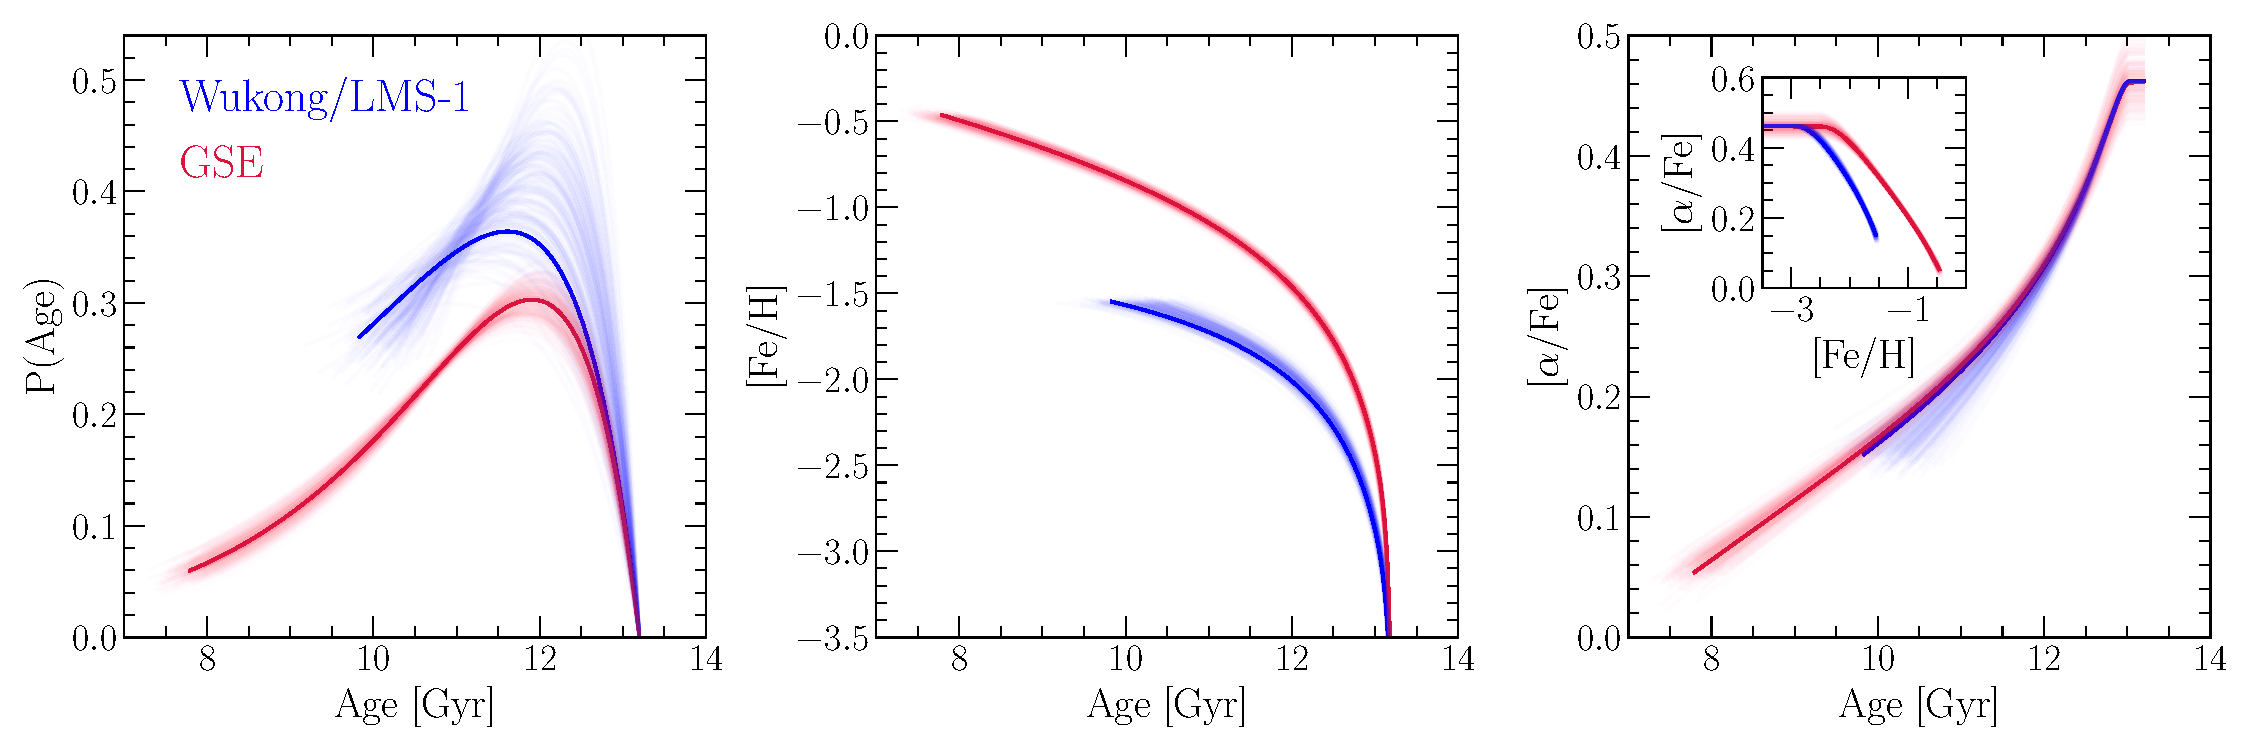
\includegraphics[scale = 0.45]{gse_wukong_comparison.pdf}
\caption{
A comparison of the predictions of our best-fit GCE models describing our
GSE (red) and Wukong (blue) data: the age distributions (left), the
age-\feh~relations (middle) and age-\afe~relations (right).
The inset in the right hand panel shows the tracks in the~\afe-\feh~plane.
In all panels, we subsample 200 additional parameter choices from our Markov
chains and plot the predictions as high transparency lines to provide a sense
of the fit uncertainty.
Due to the lack of age information for Wukong, the results in each panel with
the exception of the inset can shift left or right without impacting the
quality of the fit.
}
\label{fig:comparison}
\end{figure*}

Our sample from the Wukong stream consists of 57 stars, none of which have age
information because they are distant red giant stars.
This sample spans two orders of magnitude in metallicity, from
$\feh \approx -3.5$ to~$-2.5$.
Our GSE stars, however, have reached solar~\afe~while the least alpha-rich
Wukong star has~$\afe \approx +0.1$.
Abundance uncertainties range from~$\sim$0.02 to~$\sim$0.10 dex in
both~\afe~and~\feh~with median values near~$\sim$0.045.
\par
Fig.~\ref{fig:wukong} illustrates our sample in the~\afe-\feh~plane along with
associated marginalized distributions. There are a notable number of stars near
the ``knee'' associated with the onset of SN Ia enrichment around
$\feh \approx -3$.
Similar to the GSE but to an even greater extent, the metal-poor and alpha-rich
nature of the MDF is indicatove of slow star formation and strong outflows, and
the lack of discontinuities in the age and abundance trends indicates a smooth
SFH devoid of any starburst events.
We therefore fit our Wukong sample with the same evolutionary history as the
input model to our mock samples which we also applied to the GSE data,
retaining the assumption that the H3 selection function is uniform in chemical
space (see discussion in~\S~\ref{sec:h3:gse}).
However, because SN yields should be set by stellar physics, we fix our Fe
yields at~$\yfecc = \scinote{7.78}{-3}$ and~$\yfeia = \scinote{1.23}{-3}$ as
determined by our fit to the GSE data.
\par
Fig.~\ref{fig:wukong_corner} shows the ``corner-plot'' obtained from fitting
this model to our Wukong sample using the likelihood function given by
equation~\refp{eq:likelihood}.
The marginalized likelihood distributions are noticably asymmetric, a
consequence of degeneracies that arise in the evolutionary timescales in the
absence of age information.
We found similar effects in our mock samples with~$f_\text{age} = 0$ and in
fitting our GSE sample with no age information in~\S~\ref{sec:h3:gse}.
This fit indicates considerably stronger winds ($\sim$5 times larger~$\eta$)
and slower star formation ($\sim$3 times larger~$\tau_\star$) than the GSE.
Both of these results point to the Wukong progenitor being significantly less
massive than the GSE progenitor, which is expected since the GSE is perhaps the
most massive satellite to have merged with the Milky Way~\citep{Deason2019,
Fattahi2019, Mackereth2019, Vincenzo2019}.
Our fit additionally indicates that the Wukong progenitor experienced a more
extended infall history with an accretion timescale of
$\tau_\text{in} \approx 3.5$ Gyr compared to~$\sim$1 Gyr.
This result is in qualitative agreement with the variations in SFHs as a
function of stellar mass predicted by semi-analytic models of galaxy formation
(see, e.g., the reviews of~\citealt{Baugh2006} and~\citealt{Somerville2015a}).
\par
We plot the evolutionary track of our best-fit GCE model in the~\afe-\feh~plane
and the marginalized distributions on top of the data in Fig.~\ref{fig:wukong}.
Using equation~\refp{eq:chisquared_dof} to assess the quality of the fit,
we compute~$\chi_\text{dof}^2 = 0.98$ for this model, indicating that this is
an excellent fit to our Wukong sample.
At first glance, it may seem that our SN yields underestimate the height of the
plateau in~\afe which arises due to the IMF-averaged CCSN yields of alpha
and iron-peak elements.
To address this, we conduct one additional fit where the SN yields of Fe are
free parameters, finding~$\yfecc = \scinote{6.65}{-4}$ and
$\yfeia = \scinote{3.26}{-3}$ with the remaining evolutionary parameters
otherwise consistent to the fit with fixed yields.
We plot this model in Fig.~\ref{fig:wukong} for comparison as well, computing
$\chi_\text{dof}^2 = 0.84$.
This indicates that a slightly better fit can indeed be obtained with a higher
plateau height for Wukong than is suggested by our GSE sample, but both are
statistically excellent fits anyway.
\par
In Fig.~\ref{fig:comparison}, we compare our best-fit models for the GSE and
Wukong progenitors.
The intrinsic age distribution of GSE is predicted with considerably higher
precision than for Wukong, a consequence of the lack of age information in our
Wukong data.
The uncertainties in the Wukong age distribution are noticably asymmetric due
to non-uniform confidence intervals in the inferred evolutionary timescales.
If our assumption that star formation began~$T \approx 13.2$ Gyr ago (see
discussion in~\S~\ref{sec:mocks:fiducial}) is accurate for Wukong, then it
experienced quenching~$\sim$2 Gyr earlier than the GSE ($\sim$9.8 versus
$\sim$7.8 Gyr ago).
However, because we do not have age information for Wukong, this distribution
could shift uniformly to significantly lower values with affecting the quality
of the fit at all (that is, given only knowledge of the abundances without
incorporating any information from the Wukong CMD).
Furthermore, given the discrepancies between our fit to the GSE data with and
without the individual age measurements (see discussion at the end
of~\S~\ref{sec:h3:gse}), we expect that the timescales inferred by our fit
may change if we were to incorporate either individual age measurements or an
empirically-motivated prior on the SFH into our fit to the Wukong stream.
\par
Again as a consequence of the lack of age information, the intrinsic
age-\feh~and age-\afe~relations achieve noticable higher precision for GSE
than Wukong.
While the age-\feh~relations are significantly offset from one another due to
differences in their equilibrium abundances, the predicted age-\afe~relations
are remarkably consistent with one another.
A portion of this agreement can likely be traced back to our fixing the Fe
yields in our fit to Wukong to the values inferred in our fit to GSE.
Nonetheless, it is reasonable to assume that the SN yields are the same between
the two galaxies because this should be set by stellar physics, sufficiently
decoupled from the galactic environment.
The evolution of~\afe~with time is in principle impacted by the various
evolutionary timescales at play, so their consistency with one another is still
noteworthy.

\end{document}
